%%%%%%%%%%%%%%%%%%%%%%%%%%%%% Define Article %%%%%%%%%%%%%%%%%%%%%%%%%%%%%%%%%%
\documentclass{article}
%%%%%%%%%%%%%%%%%%%%%%%%%%%%%%%%%%%%%%%%%%%%%%%%%%%%%%%%%%%%%%%%%%%%%%%%%%%%%%%

%%%%%%%%%%%%%%%%%%%%%%%%%%%%% Using Packages %%%%%%%%%%%%%%%%%%%%%%%%%%%%%%%%%%
\usepackage{geometry}
\usepackage{graphicx}
\usepackage{amssymb}
\usepackage{amsmath}
\usepackage{amsthm}
\usepackage{empheq}
\usepackage{mdframed}
\usepackage{booktabs}
\usepackage{lipsum}
\usepackage{graphicx}
\usepackage{color}
\usepackage{psfrag}
\usepackage{pgfplots}
\usepackage{bm}
%%%%%%%%%%%%%%%%%%%%%%%%%%%%%%%%%%%%%%%%%%%%%%%%%%%%%%%%%%%%%%%%%%%%%%%%%%%%%%%

% Other Settings

%%%%%%%%%%%%%%%%%%%%%%%%%% Page Setting %%%%%%%%%%%%%%%%%%%%%%%%%%%%%%%%%%%%%%%
\geometry{a4paper}

%%%%%%%%%%%%%%%%%%%%%%%%%% Define some useful colors %%%%%%%%%%%%%%%%%%%%%%%%%%
\definecolor{ocre}{RGB}{243,102,25}
\definecolor{mygray}{RGB}{243,243,244}
\definecolor{deepGreen}{RGB}{26,111,0}
\definecolor{shallowGreen}{RGB}{235,255,255}
\definecolor{deepBlue}{RGB}{61,124,222}
\definecolor{shallowBlue}{RGB}{235,249,255}
%%%%%%%%%%%%%%%%%%%%%%%%%%%%%%%%%%%%%%%%%%%%%%%%%%%%%%%%%%%%%%%%%%%%%%%%%%%%%%%

%%%%%%%%%%%%%%%%%%%%%%%%%% Define an orangebox command %%%%%%%%%%%%%%%%%%%%%%%%
\newcommand\orangebox[1]{\fcolorbox{ocre}{mygray}{\hspace{1em}#1\hspace{1em}}}
%%%%%%%%%%%%%%%%%%%%%%%%%%%%%%%%%%%%%%%%%%%%%%%%%%%%%%%%%%%%%%%%%%%%%%%%%%%%%%%

%%%%%%%%%%%%%%%%%%%%%%%%%%%% English Environments %%%%%%%%%%%%%%%%%%%%%%%%%%%%%
\newtheoremstyle{mytheoremstyle}{3pt}{3pt}{\normalfont}{0cm}{\rmfamily\bfseries}{}{1em}{{\color{black}\thmname{#1}~\thmnumber{#2}}\thmnote{\,--\,#3}}
\newtheoremstyle{myproblemstyle}{3pt}{3pt}{\normalfont}{0cm}{\rmfamily\bfseries}{}{1em}{{\color{black}\thmname{#1}~\thmnumber{#2}}\thmnote{\,--\,#3}}
\theoremstyle{mytheoremstyle}
\newmdtheoremenv[linewidth=1pt,backgroundcolor=shallowGreen,linecolor=deepGreen,leftmargin=0pt,innerleftmargin=20pt,innerrightmargin=20pt,]{theorem}{Theorem}[section]
\theoremstyle{mytheoremstyle}
\newmdtheoremenv[linewidth=1pt,backgroundcolor=shallowBlue,linecolor=deepBlue,leftmargin=0pt,innerleftmargin=20pt,innerrightmargin=20pt,]{definition}{Definition}[section]
\theoremstyle{myproblemstyle}
\newmdtheoremenv[linecolor=black,leftmargin=0pt,innerleftmargin=10pt,innerrightmargin=10pt,]{problem}{Problem}[section]
%%%%%%%%%%%%%%%%%%%%%%%%%%%%%%%%%%%%%%%%%%%%%%%%%%%%%%%%%%%%%%%%%%%%%%%%%%%%%%%

%%%%%%%%%%%%%%%%%%%%%%%%%%%%%%% Plotting Settings %%%%%%%%%%%%%%%%%%%%%%%%%%%%%
\usepgfplotslibrary{colorbrewer}
\pgfplotsset{width=8cm,compat=1.9}
%%%%%%%%%%%%%%%%%%%%%%%%%%%%%%%%%%%%%%%%%%%%%%%%%%%%%%%%%%%%%%%%%%%%%%%%%%%%%%%

%%%%%%%%%%%%%%%%%%%%%%%%%%%%%%% Title & Author %%%%%%%%%%%%%%%%%%%%%%%%%%%%%%%%
\title{Apuntes de practicas}
\author{Rodrigo Miranda}
%%%%%%%%%%%%%%%%%%%%%%%%%%%%%%%%%%%%%%%%%%%%%%%%%%%%%%%%%%%%%%%%%%%%%%%%%%%%%%%

\begin{document}
    \maketitle
    Ejemplos de practica AMN941  - Usando Latex en VSCode
    \section*{Metodo del punto}Use el método de punto para encontrar una raíz real de la ecuación
    \[
        f(x)= x^{3}+2x^{2}+10x-20 =0
        \]
    Empleando como valor inicial $x0=1$. Emplee $15$ decimales y una precisión de $10^{-5}$.


    \textbf{Solucion:} 

    \noindent Para punto fijo, debemos obtener una ecuacion $g(x)=x$ 


    \textbf{Opcion 1:} $x= x^{3}+2x^{2}+11x-20$
    
    \noindent \\ Verificamos que la ecuacion converga en el punto dado, para ello derivamos la ecuacion $g(x)$ y evaluamos en el punto, de manera que:

    $g'(x)=3x^{2}+4x+11 \longrightarrow g'(1)=18$

    \noindent \\ Esto lo podemos comprobar rapidamente tambien en matlab, de la siguiente manera
    \begin{figure}[ht]
        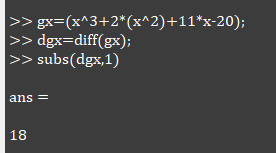
\includegraphics[scale=1]{img/ejemplo_clasePunto.png}
        \caption[Derivada y evaluacion g'(x)]{Matlab 1}
    \end{figure}
    \\Por lo tanto, incumplimos el teorema de Banach quien expresa que $|g'(x)|<1$ \pagebreak
    
    \textbf{Opcion 2: }$\frac{20}{x^2+2x+10}$
    \noindent \\Probamos esta ecuacion y derivada evaluada en matlab
    \begin{figure}[ht]
        \includegraphics*[scale=0.9]{img/ejemplo_clasePunto_2.png}
        \caption[Derivada y evaluacion g'(x)]{Matlab 2}
    \end{figure}
    \\Como podemos observar, el resultado de la evaluacion es menor a 1, por lo tanto si converge.

    \noindent Probaremos esta ecuacion con el metodo de punto fijo en Matlab.
    \begin{figure}[ht]
        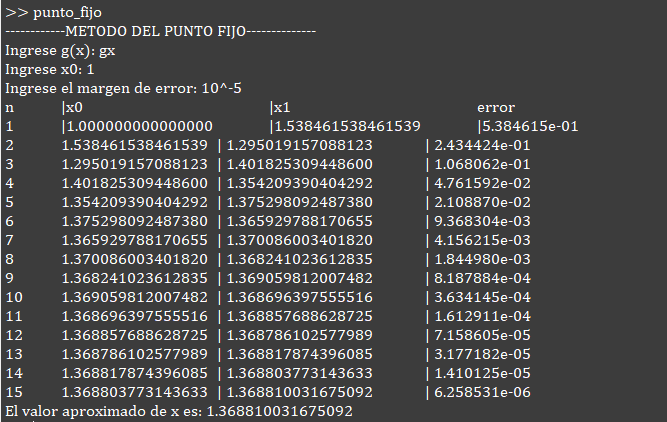
\includegraphics[scale=0.9]{img/ejemplo_clasePunto_3.png}
        \caption[Metodo Punto Fijo]{Matlab 3}
    \end{figure}
    \\El valor aproximado de $x=1.368810031675092$


    \section*{Newton}Use el método de Newton - Raphson para encontrar una solución exacta con una exactitud de $10^{-12}$ para la siguiente ecuación. Emplee 15 decimales: 
    \[
        \ln(x-1)+cos(x-1)=0 ; [1.3,2]
    \]
    \begin{figure}[ht]
        \includegraphics*[scale=0.9]{img/ejemplo3.png}
    \end{figure}
    
    
    
    
\end{document}